\documentclass[french]{article}
\usepackage[T1]{fontenc}
\usepackage[utf8]{inputenc}
\usepackage{lmodern}
\usepackage{graphicx}
\usepackage[a4paper,left=3cm,right=3cm,top=2.5cm,bottom=2.5cm]{geometry}
\usepackage{babel}

\usepackage{fancyhdr}
\pagestyle{fancy}
\renewcommand{\headrulewidth}{1pt}
\fancyhead[L]{Algorithmique et Programmation Avancée}
\fancyfoot[R]{Ebersold, Thieblin, Desprat}
\fancyhead[R]{Département Mathématiques-Informatique}
\fancyfoot[L]{MIA0301V - MI00304}


\usepackage{listingsutf8}
\usepackage{listings}
\usepackage{xcolor}
\lstset { %
	language=C++,
    basicstyle=\footnotesize\ttfamily,
    keywordstyle=\color{blue}\ttfamily,
    stringstyle=\color{red}\ttfamily,
    commentstyle=\color{olive}\ttfamily,
    morecomment=[l][\color{magenta}]{\#},
	backgroundcolor=\color{black!5}, % set backgroundcolor
	numbers=left, 
    numberstyle=\tiny\ttfamily, 
    breaklines=true,
    numbersep=5pt,
    xleftmargin=.25in,
    xrightmargin=.25in
}
\lstset{%
	inputencoding=utf8,
	extendedchars=true,
	literate=%
	{é}{{\'e}}{1}%
	{è}{{\`e}}{1}%
	{à}{{\`a}}{1}%
	{ç}{{\c{c}}}{1}%
	{œ}{{\oe}}{1}%
	{ù}{{\`u}}{1}%
	{É}{{\'E}}{1}%
	{È}{{\`E}}{1}%
	{À}{{\`A}}{1}%
	{Ç}{{\c{C}}}{1}%
	{Œ}{{\OE}}{1}%
	{Ê}{{\^E}}{1}%
	{ê}{{\^e}}{1}%
	{î}{{\^i}}{1}%
	{ô}{{\^o}}{1}%
	{û}{{\^u}}{1}%
	{ë}{{\¨{e}}}1
	{û}{{\^{u}}}1
	{â}{{\^{a}}}1
	{Â}{{\^{A}}}1
	{Î}{{\^{I}}}1
}


\begin{document}
	
	\begin{minipage}{\textwidth}
\begin{center}

{\Large Mise en œuvre avec C++ \\ Feuille d'exercices : \textbf{Recherches et tris}}
\end{center}
	\end{minipage}
	
\section*{Rappel}
En C++, il est nécessaire d'avoir un (et un seul) sous-programme \texttt{main} -- qui renvoit toujours un entier -- à partir duquel s'exécute les sous-programme. On l'écrit dans un fichier \texttt{.cpp} préalablement créé.
\begin{lstlisting}[caption={Exemple de main dans recherche1.cpp}]
int main(){
    //appel des sous programmes
    //...
    cin.get();//attendre que l'utilisateur appuie sur ENTREE
    return 0;
}    
\end{lstlisting}

\section*{Sous programme supplémentaires}
	\begin{lstlisting}[caption={Sous programmes supplémentaires}]
//remplir un tableau
void remplirTableau(int tab[], int taille){
    //...
}

//afficher un tableau
void afficherTableau(int tab[], int taille){
    //...
}


int main(int argc, char *argv[])
{
    int taille=4;
    int tab[taille];
    remplirTableau(tab,taille);
    int val=6;
    
    //appels de recherche_1 non trie 
    //...
    
    //appels des differents tris
    //...
    
    //appels des differentes recherches sur tableau trie
    //...
    
    cin.get();//attendre l'utilisateur
    return EXIT_SUCCESS;
}
\end{lstlisting}
\section{Recherche d'un élément dans un tableau}

	$\rightarrow$ Au sein d’un programme \texttt{recherche\_1.cpp}, écrire un sous-programme qui prend en paramètres un tableau non trié et une valeur à rechercher, et qui retourne l’indice de l’élément recherché à l’intérieur du tableau s’il existe, -1 sinon.
	
\section{Recherche d'un élément dans un tableau trié}
	$\rightarrow$ Même question pour un \textbf{tableau trié} \texttt{recherche\_2.cpp}.
	\section{Recherche d'un élément dans un tableau trié par dichotomie}
	
	\begin{figure}[h]
		\centering
		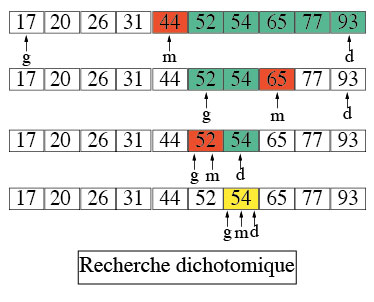
\includegraphics[width=0.4\textwidth]{dicho.jpg}
	\end{figure}
	$\rightarrow$ Même question pour un tableau trié, mais la recherche doit se faire par \textbf{dichotomie} \texttt{recherche\_3.cpp}
\section{Tri par insertion}

\subsection*{Exemple}
Tri utilisé quand on classe des factures par date. On prend une facture et on le met à sa place parmi les factures déjà triées. Puis on recommence avec la facture suivante. 

\subsection*{Principe}
\begin{enumerate}
	\item Parcourir un tableau dans l'ordre des éléments
	\item Les comparer avec les éléments précédents jusqu'à trouver la place de l'élément qu'on considère.
	\item Décaler les éléments du tableau pour insérer l'élément considéré à sa place dans la partie déjà triée
\end{enumerate} 
Pour procéder à un \textbf{tri par insertion}, il suffit de parcourir un tableau : on prend les éléments dans l'ordre. Ensuite, on les compare avec les éléments précédents jusqu'à trouver la place de l'élément qu'on considère. Il ne reste plus qu'à décaler les éléments du tableau pour insérer l'élément considéré à sa place dans la partie déjà triée

\subsection*{A faire}
 Au sein d’un programme \texttt{tri\_insertion.cpp}, écrire un sous-programme qui prend en paramètre un tableau quelconque et le retourne trié. Le tri se fait selon la méthode de l’insertion. 
\begin{enumerate}
	\item Créer le fichier \texttt{tri\_insertion.cpp}
	\item Écrire un sous-programme qui prend en paramètre un tableau quelconque et le retourne trié (\textbf{par insertion}).
\end{enumerate}

\section{Tri par sélection}

\subsection*{Principe}

Même problème en utilisant un tri par sélection. Le \textbf{tri par sélection} consiste en la recherche soit du plus grand élément (ou le plus petit) que l'on va replacer à sa position finale c'est-à-dire en dernière position (ou en première), puis on recherche le second plus grand élément (ou le second plus petit) que l'on va replacer également à sa position finale c'est-à-dire en avant- dernière position (ou en seconde), etc., jusqu'à ce que le tableau soit entièrement trié.
\begin{enumerate}
	\item Rechercher le plus grand élément dans le tableau
	\item Le replacer à sa position finale i.e. en dernière position.
	\item Recherche le second plus grand élément
	\item Le replacer à sa position finale i.e. en avant-dernière position.
	\item etc... jusqu'à ce que le tableau soit entièrement trié.
\end{enumerate} 
\subsection*{A faire}
\begin{enumerate}
	\item Créer le fichier \texttt{tri\_selection.cpp}
	\item Écrire un sous-programme qui prend en paramètre un tableau quelconque et le retourne trié (\textbf{par sélection}).
\end{enumerate}
\section{Tri à bulles}

\subsection*{Principe}
Même problème en utilisant un tri à bulles. Le \textbf{tri à bulles} consiste à faire remonter le plus grand élément du tableau (comme une bulle d'air remonte à la surface) en comparant les éléments successifs. C'est-à-dire qu'on va comparer le 1er et le 2e élément du tableau, conserver le plus grand et puis les échanger s'ils sont désordonnés les uns par rapport aux autres. On recommence cette opération jusqu'à la fin du tableau. Ensuite, il ne reste plus qu'à renouveler cela jusqu'à l'avant-dernière place et ainsi de suite...

\begin{enumerate}
	\item \textbf{Comparer} le 1er et le 2e élément du tableau et \textbf{conserver} le plus grand et puis les échanger s'ils sont désordonnés les uns par rapport aux autres.
	\item Recommencer l'opération 1 jusqu'à la fin du tableau.
	\item Renouveler l'opération 2 jusqu'à l'avant-dernière place et ainsi de suite.
\end{enumerate} 
\subsection*{A faire}
\begin{enumerate}
\item Créer le fichier \texttt{tri\_bulle.cpp}
\item Écrire un sous-programme qui prend en paramètre un tableau quelconque et le retourne trié avec (\textbf{un tri à bulles}).
\end{enumerate}
\end{document}
